\documentclass[12pt,a4paper]{article}

\makeatletter
\def\input@path{{/home/maenwe/Master_CSM/modèle_cours_latex}}
\makeatother

\usepackage{prise_de_note}
\graphicspath{{images}}
\begin{document}
	\pagenumbering{gobble}
	\begin{titlepage}
		\centering
		
		% Logo
		\begin{figure}[h]
			\centering
			% Ajustez la largeur si besoin (ex: 0.4 ou 0.6)
			
\includegraphics[width=0.5\textwidth]{/home/maenwe/Master_CSM/modèle_cours_latex/logo.jpg} 
		\end{figure}
		
		\vspace{2cm}
		
		% Filet horizontal du haut
		\rule{\linewidth}{0.5mm} \\[0.4cm]
		
		% Titre
		{\color{bleuTitre} \Huge \bfseries Phénomène de propagation} \\[0.4cm]
		
		% Filet horizontal du bas
		\rule{\linewidth}{0.5mm}
		
		\vspace{1.5cm}
		
		{\Large \textbf{Cours}}
		
		\vfill
		
		% Bloc Informations
		\begin{minipage}{0.45\textwidth}
			\begin{flushleft} \large
				\textbf{Enseignant :} \\
				M. Benjamin \textsc{BOUTIN}\\
				M. François \textsc{CASTELLA}
			\end{flushleft}
		\end{minipage}
		\hfill
		\begin{minipage}{0.45\textwidth}
			\begin{flushright} \large
				\textbf{Étudiant :} \\
				Nathan \textsc{HASCOET}
			\end{flushright}
		\end{minipage}
		
		\vspace{2cm}
		
		% Date
		{\large \today}
		
	\end{titlepage}
	
	\tableofcontents
	
	\newpage
	\pagenumbering{arabic}
	\setcounter{page}{1}
	
	\part{Cours M. Boutin}
	\section{Introduction aux problèmes de propagation}
	\subsection{Discussion}
	
	\textbf{\textcolor{red}{Attention !}} propagation $\not=$ déplacement de matière.\\
	On étudie l'évolution d'une quantité par rapport à un état de référence.
	
	\begin{ex}
		\begin{minipage}[t]{15cm}
			\begin{enumerate}[label=\textbullet]
			\item Corde de guitare, équation des ondes 1D (en première approximation)
			
			\item  radar, one électromagnétiques.
			
			\item sonar, échographie : ondes acoustiques dans un fluide
			
			\item  sismologie, elastodynamie en milieu solide complexe
			
			\item houle, tsunamies : ondes de surface (déformation de surface libre)
			
			\item trafic routier : véhicules en mouvement et leur densité  $\to$ modélisation fluide
		\end{enumerate}
		\end{minipage}
	\end{ex}
	
	
	les ondes propagées peuvent faire l'objet :
	\begin{enumerate}[label=$-$]
		\item réflexion et transmission(interfaces et bords)
		
		\item réfraction
		
		\item dispersion : les vitesses de propagation peuvent différer d'une solution à l'autre et êre modifiée dans le temps (l'onde se déforme)
		
		\item  amortissement ou amplification de l'onde.
	\end{enumerate}
	 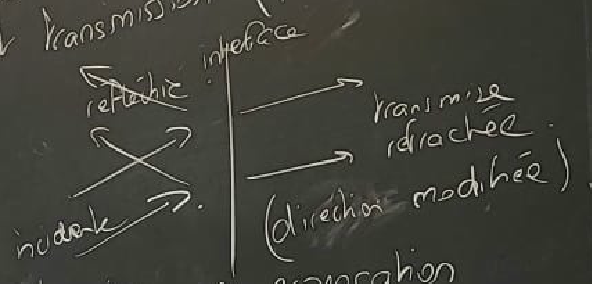
\includegraphics[scale=.3]{im1.png}


	\subsection{Modèles}
	
	\subsubsection{Advection d'un polluant}
	
	Concentration $c(t,x)>0$ de polluant dans un champ de vitesse $u(t,x \in \R$, $x \in \R$ la position dans l'espace.\\
	$\to$ \underline{flux d'advection} du polluant $F(t,x) = u(t,x)c(t,x)$.\\
	bilan local de \underline{particules}\hspace*{.5cm} \begin{minipage}{15cm}
		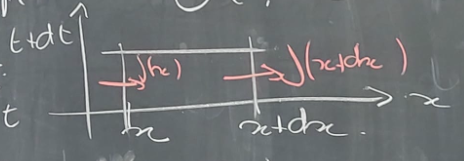
\includegraphics[scale=.3]{im2.png}
	\end{minipage}\\
	$c(t+\dt)\dx = c(t)\dx+F(t,x)\dt-D(x+\dx)\dt \underset{\text{sol. reg.}}\to \fbox{$\partial_t c + \partial_x D = 0.$}$\\
	
	Si on tient compte d'un éventuel flux de diffusion : \underline{loi de Fick :} $D_{diff} = -D\partial_x c$ ($D$ est une constante de diffusion moléculaire \fbox{$D>0$}).L'équation d'advecion diffusion est alors : 
	\begin{equation}
		\partial_t c + \partial_x(uc) = D\partial_x^2 c,
	\end{equation}
	c'est une équation de conservation (issue d'un bilan local conservatif). En dimension suérieure, la dérivation de l'équation repose sur la formle de Green pour $u(t,x) \in \R^3$ :
	\begin{equation}
		\partial_t c + \mathrm{div}_{\underbrace{(x,y,z)}_{\vec x}} (uc) = \underbrace{\mathrm{div}_{\vec x}\left(D\nabla_{\vec x} c\right)}_{D\text{ indep. de } (\vec x, t) : D\Delta c}
	\end{equation}
	
	\begin{minipage}{5cm}
		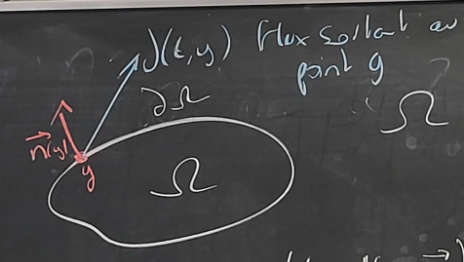
\includegraphics[scale=.3]{im3.png}
	\end{minipage} $\Omega$ élément de volume dans $\R^3$.
	
	\[
		c(t+\mathrm d\vec x)\mathrm{Vol}(\Omega) = c(t,\vec x)\textsc{Vol}(\Omega) - \underbrace{\int_{\partial\Omega} \left(\vec D(t,\vec y)\cdot\vec n (\vec y)\right) \mathrm d\sigma(\vec y)\dt}_{=\int_\Omega \mathrm{div}\vec D\mathrm d\vec x}
	\]
	\[
		\int_\Omega \left[\dfrac{c(t+\dt,\vec x)-c(t,\vec x)}{\dt}+\mathrm{div}D\right]\mathrm d\vec x = 0
	\]
	Il suit :
	\begin{equation}
		\partial_t c + \mathrm{div} D = 0,
	\end{equation}
	(advection "passive" : $u$ ne dépend pas de $c$).
	
	Si $u$ est constante et uniforme, on a : $\underbrace{\partial_t c + u\partial_x c = 0}{\text{eq. de transpor à viesse }u}$  pour le cas 1D sans diffusion.\\
	De façon générale : $\partial_x(uc) = u\partial_x c + c\partial_x u$, donc : $\partial_t c + u\partial_x c = -(\partial_x u) c$ : induit une amplification ou réduction de $c$ le long de certaines courbes.\\
	
	A contrario, si $\partial_x u=0$, c'est une constante le long de certaines courbes.
	
	\subsubsection{Modèles d'équations d'ondes}
	
	$\to$ \underline{Corde endue de masse linéique $\rho$, tension $T$.}
	
	\begin{center}
		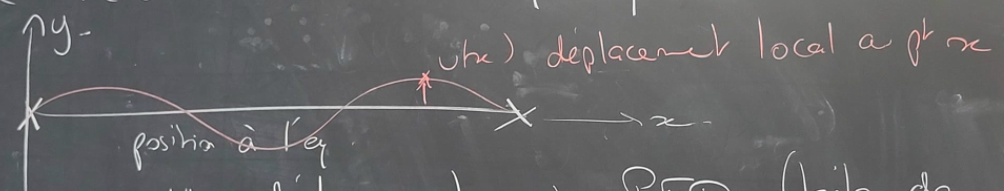
\includegraphics[scale=.3]{im4.png}
	\end{center}
	
	sous hypothèse de petits déplacements et PFD (bilan de forces) :
	\begin{equation}
		\rho \dfrac{\partial^2u}{\partial t^2} = T\dfrac{\partial^2 u}{\partial x^2}
	\end{equation}
	la déformation $u$ se propage le long de la corde.\\
	
	$\to$ \underline{Equation de Maxwell pour l'électromagnétisme}\\
	Champ électrique $\vec E(t,\vec x) \in \R^3$, magnétique $\vec H(t,\vec x) \in \R^3$, induction électrique $\vec D(t,\vec x) \in \R^3$, magnétique $\vec B(t,\vec x) \in \R^3$. En l'absence de charge et courant ("dans le vide")*.\\
	\begin{minipage}[t]{.5\textwidth}
		\textcolor{red}{bilan}$\begin{cases}
			\dfrac{\partial \vec B}{\partial t} = - \vec{\mathrm{rot}}\vec E \\
			\dfrac{\partial\vec D}{\partial t} = \vec{\mathrm{rot}} \vec H
		\end{cases}$\\
		\textcolor{red}{vide "géométrique} $\begin{cases}
			\mathrm{div}\vec D = 0\\
			\mathrm{div} \vec D = 0
		\end{cases}$
	\end{minipage}\begin{minipage}[t]{.5\textwidth}
	\textcolor{red}{loi de comportement.}\\
	$\vec B = \mu \vec H$ : perméabilité magnétique\\
	$\vec D = \varepsilon \vec E$ : permittivité diélectrique du vide.
	\end{minipage}
	
	En combinant les équations (une sorte d'"élimination de Gauss"), il suit : 
	\[\begin{cases}
		\dfrac{\partial \vec H}{\partial t} = -\dfrac1\mu\vec{\mathrm{rot}}\vec E\\
		\varepsilon\dfrac{\partial\vec E}{\partial t} = \vec{\mathrm{rot}} \vec H
	\end{cases}\]
	, ainsi par élimination:
	\begin{equation}
		\varepsilon\dfrac{\partial^2 \vec E}{\partial t^2} + \vec{\mathrm{rot}}\left(\dfrac1\mu\vec{\mathrm{rot}}\vec E\right) = 0.
	\end{equation}
	Si $\varepsilon$ et $\mu$ sont constants, $\vec{\mathrm{rot}}(\vec{\mathrm{rot}} \vec E) = \vec\nabla\left(\underbrace{\nabla\cdot\vec E}_{=0}\right) - \vec\Delta\vec E$. On obtient finalement :
	
	\begin{equation}
		\dfrac{\partial^2 \vec E}{\partial t^2} - c^2\vec\delta\vec E = 0,
	\end{equation}
	avec $c = \dfrac1{\sqrt{\varepsilon\mu}}$.		
	\subsubsection{Modèle de trafic routier (LWR)}
	LWR = Lightill, Whitham, Richards.\\
	Route unidimensionelle $x \in \R$, temps $t>0$.\\
	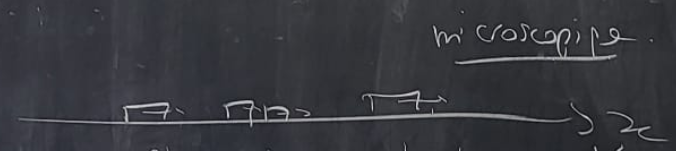
\includegraphics[scale=.5]{im5.png}\\
	véhicule en file indienne le long de l'axe (sans dépassements ni jonctions).\\
	modèle fluide : \begin{minipage}[t]{15cm}
		$\rho(tnx)$ densité de véhicule autour de $x$,\\
		 $v(,x)$ vitesse moyenne autour du point $x$,\\
		  flux de véhicule : $q(t,x) = \rho(,x)v(t,x)$.
	\end{minipage}
	
	\underline{bilan de masse} sur un intervalle $[a;b]$.\\
	$N(t) = \displaystyle\int_a^b\rho(t,x)\dx$\\
	$\dfrac{d}{\dt}N(t) = q(t,b) - q(t,a) = \displaystyle\int_a^b\partial_x q(t,y) \dy$, d'où $\displaystyle\int_a^b \left(\partial_t\rho + \partial_x q\right)\dy = 0$, ceci pour tout $(a,b)$. Donc :
	\begin{equation}
		\partial_t \rho + \partial_x q = 0.
	\end{equation}
	On se donne une loi de comportement : $v = V(\rho)$ avec $V$ une fonction prescrite.\\
	\underline{typiquement :} $ V(\rho) = V_{\max}\left(1-\dfrac\rho{\rho_{\max}}\right)$. On a :
	\begin{equation}
		\partial_t \rho + \partial_x\left(\underbrace{\rho V(\rho)}_{Q(\rho)}\right) = 0,
	\end{equation}
	équation de transport conservative mais non-linéaire.
	
	
	\begin{center}
		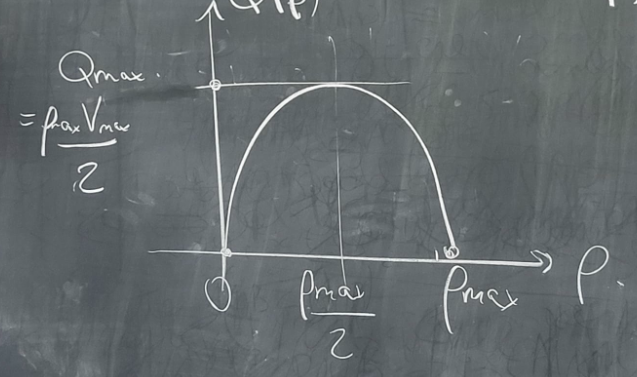
\includegraphics[scale=.3]{im6.png}
	\end{center}
	
	\begin{rmq}
		si $\rho$ est solution régulière :
		\begin{equation}
			\partial_t \rho + Q'(\rho)\partial_x \rho = 0,
		\end{equation}
		on en déduit ainsi l'équation suivante : 
		\[Q'(\rho) = V(\rho) + \rho V'(\rho) = V_{\max}\left(1-\dfrac\rho{\rho_{\max}}\right)-\rho\dfrac{V_{\max}}{\rho_{\max}} = V_{\max} \left(1-2\rho/\rho_{\max}\right)\]
		vitesse de propagation des fluctuations de $\rho$ :
		\begin{enumerate}[label=$ $]
			\item  $> 0$ si : $\rho < \rho_{\max}/2$
			\item $<0$ si $\rho>\rho_{\max}/2$
		\end{enumerate}
		tandis que les véhicules ont toujours la vitesse $V(\rho) >0$.
	\end{rmq}
\end{document}